\chapter{ESTUDIO EXPERIMENTAL}
\label{chap:estudio_experimental}

\section{Introducción}
\label{sec:exp_introduccion}

La agricultura moderna busca producir más alimentos de forma sostenible, adoptando prácticas que optimicen el uso del recurso hídrico \shortcite{Laveglia2024, Vargas2021}. Una estrategia fundamental para lograrlo es la agricultura de precisión que mide y responde a la variabilidad de los cultivos para mejorar su manejo \shortcite{Dong2024, Pineda2021}. Pero la implementación de técnicas avanzadas como la termografía infrarroja (en adelante IRT), un método no invasivo y eficaz para detectar estrés hídrico a través de la temperatura foliar \shortcite{GarciaTejero2015, Pineda2021}, ha sido limitada por el alto costo de los equipos comerciales \shortcite{Dong2024, Salgado2018}. Por lo tanto, existe una brecha tecnológica que frena su adopción, haciendo necesario el desarrollo de herramientas de monitoreo asequibles que democraticen el acceso a estas tecnologías.

En este escenario, el arándano (\textit{Vaccinium corymbosum} L.) se destaca como la cuarta frutilla de mayor importancia económica a nivel mundial \shortcite{Salgado2018}. En el altiplano cundiboyacense, la variedad Biloxi está en expansión \shortcite{QuintanaReina2020}, aunque su sistema radicular superficial y poco eficiente la hace altamente vulnerable al déficit hídrico, afectando crecimiento, calibre de frutos y rendimiento \shortcite{Morales2017, Almutairi2021}.

Cuando las plantas enfrentan déficit de agua, cierran estomas, reducen la transpiración y elevan su temperatura foliar, un indicador temprano del estrés hídrico \shortcite{GarciaTejero2015, Kappes2024, Vieira2021}. La IRT permite detectar este fenómeno al registrar la radiación térmica de la planta y, mediante el índice de estrés hídrico del cultivo (CWSI por sus siglas en inglés), cuantificar el nivel de afectación \shortcite{Aux2022, Jimenez2021}.

Recientes avances en hardware accesible han demostrado ser una alternativa prometedora para monitorear la temperatura foliar con suficiente precisión \shortcite{Dong2024}. En este contexto, la implementación de una prueba de concepto (PoC) se presenta como un paso metodológico crucial. Esta prueba se define como un estudio a escala reducida diseñado para demostrar la funcionalidad de una tecnología y verificar la factibilidad de un concepto antes de su desarrollo a gran escala \shortcite{Battaglia2021}.

Por esto, considerando la susceptibilidad del arándano Biloxi al estrés hídrico, este estudio se plantea como realizar una prueba de concepto orientada a desarrollar un sistema de termografía de bajo costo para la detección temprana de estrés hídrico. El objetivo es demostrar la sensibilidad del sistema para registrar cambios térmicos que sean plausibles y coherentes con el estado hídrico de la planta, aportando así una base inicial para futuros estudios agronómicos a mayor escala.

\section{Materiales y métodos}
\label{sec:exp_materiales_metodos}

\subsection{Planteamiento metodológico}
\label{subsec:exp_planteamiento}

Este estudio se diseñó como una prueba de concepto (PoC) para evaluar un sistema de monitoreo de bajo costo \shortcite{Battaglia2021, Pineda2021}. Para ello, se empleó un diseño de caso único ($n=1$) con una planta de arándano (var. Biloxi) de 18 meses en un microinvernadero ($120 \times 50 \times 50$ cm) en Madrid, Cundinamarca, Colombia, durante 55 días.

El objetivo fue determinar si el sistema era lo suficientemente sensible para detectar los cambios térmicos esperados durante un ciclo de estrés-recuperación, utilizando la planta como su propio control. Este diseño es coherente con el enfoque de PoC, cuyo propósito es establecer la viabilidad funcional del sistema antes de su implementación en estudios con diseños estadísticos más complejos y robustos \shortcite{Battaglia2021, Pineda2021}. Además, se realizaron observaciones cualitativas del vigor de la planta (turgencia de hojas) para contextualizar los datos cuantitativos \shortcite{Salgado2018, Yu2015, Almutairi2021}.

\section{Diseño experimental}
\label{sec:exp_diseno}

El experimento se diseñó como una prueba de concepto para evaluar la capacidad del sistema en el monitoreo de un solo individuo de arándano (var. Biloxi).
\begin{description}
    \item[Sujeto experimental:] Se utilizó una planta de arándano de la variedad Biloxi, de 18 meses de edad, una de las más cultivadas en la región \shortcite{QuintanaReina2020}. La planta se mantuvo en un microinvernadero para aislarla de condiciones ambientales exetrnas como la lluviam, neblina y el sol directo.
    \item[Ubicación y duración:] El estudio se llevó a cabo durante 55 días consecutivos, entre agosto y octubre de 2025, en el municipio de Madrid, Cundinamarca, Colombia.
    \item[Tratamiento de estrés hídrico:] El experimento se dividió en tres fases secuenciales sobre la misma planta, utilizándola como su propio control:
        \begin{enumerate}
           \item \textbf{Fase de estrés hídrico inducido:} Se suspendió completamente el riego con el fin de provocar un estado de estrés hídrico progresivo en la planta, permitiendo evaluar la sensibilidad del sistema ante la disminución del contenido de agua foliar.
            \item \textbf{Fase de recuperación:} Posteriormente, tras dos semanas de estrés inducido, se reanudó el riego de manera normal para analizar la capacidad de recuperación de la planta y la respuesta del sistema de monitoreo durante el restablecimiento hídrico.
        \end{enumerate}
\end{description}
El prototipo de hardware se instaló a una distancia fija de la planta, asegurando que el dosel foliar estuviera siempre dentro del campo de visión del sensor térmico MLX90640. Adicionalmente, se realizaron observaciones cualitativas periódicas del vigor de la planta (turgencia de hojas) para contextualizar los datos cuantitativos, siguiendo prácticas de evaluación agronómica \shortcite{Salgado2018, Yu2015, Almutairi2021}.

\section{Recolección y análisis de datos}
\label{sec:exp_recoleccion_analisis}

El firmware del ESP32-S3 fue programado para capturar datos de todos los sensores a intervalos regulares de 20 minutos durante los 55 días del experimento. En cada intervalo, se registraron y transmitieron en formato JSON al servidor los siguientes datos:
\begin{itemize}
    \item Una matriz completa de $32 \times 24$ (768) valores de temperatura del sensor térmico MLX90640.
    \item Temperatura ambiente (°C) y Humedad relativa (\%) del sensor DHT22.
    \item Iluminancia (lux) del sensor BH1750.
    \item Una imagen RGB de contexto capturada por la cámara de apoyo.
\end{itemize}
Estos datos fueron almacenados en la base de datos PostgreSQL para su posterior análisis, a excepción de las imágenes RGB, que se guardaron en un sistema de archivos compatible con S3 y se asociaron a los registros mediante metadatos.

El análisis de los datos se centró en la extracción de la temperatura foliar a partir de la matriz térmica y el cálculo del CWSI, siguiendo estos pasos:

\begin{enumerate}
    \item \textbf{Reducción de ruido y segmentación térmica:} 
    Para cada registro temporal, se promediaron seis capturas térmicas consecutivas (tomadas en rápida sucesión por el firmware) para minimizar el ruido inherente al sensor MLX90640. 
    Sobre la matriz promediada, se aplicó un algoritmo de segmentación espacial en Python para aislar los píxeles correspondientes exclusivamente a la canopia foliar, descartando el fondo (suelo, maceta, estructura del invernadero). 
    La temperatura foliar promedio ($T_c$ o $T_{\text{canopia}}$) se calculó únicamente a partir de estos píxeles segmentados, una práctica recomendada para mejorar la precisión \shortcite{Quezada2020,Vieira2021}.

    \item \textbf{Cálculo del índice de estrés hídrico (CWSI):} 
    Se utilizó la metodología empírica del CWSI, desarrollada originalmente por Idso et al. \shortcite{Idso1981}, que normaliza la diferencia entre la temperatura del dosel ($T_c$) y la temperatura del aire ($T_a$) utilizando referencias teóricas para las temperaturas foliares en condiciones de máxima transpiración ($T_{\text{wet}}$) y mínima transpiración ($T_{\text{dry}}$). 
    El índice se calculó utilizando la siguiente fórmula \shortcite{Quezada2020}:

    \[
    \text{CWSI} = \frac{(T_c - T_a) - (T_{\text{wet}} - T_a)}{(T_{\text{dry}} - T_a) - (T_{\text{wet}} - T_a)}
    \]

    donde $(T_{\text{wet}} - T_a)$ representa el límite inferior (enfriamiento máximo) y $(T_{\text{dry}} - T_a)$ el límite superior (sin enfriamiento), ambos estimados a partir de modelos teóricos o líneas base empíricas \shortcite{Quezada2020,Aux2022}. 
    En este estudio, se implementó un método de cálculo empírico con líneas base horarias para $T_{\text{wet}}$ y $T_{\text{dry}}$, buscando mitigar las variaciones térmicas naturales entre el día y la noche. 
    Un valor de CWSI cercano a 0 indica ausencia de estrés, mientras que un valor cercano a 1 indica estrés hídrico severo.

    \item \textbf{Análisis de tendencias y correlación ambiental:} 
    Los datos de $T_c$, $\Delta T = T_c - T_a$, y CWSI se graficaron a lo largo del tiempo para visualizar las tendencias durante las dos fases del experimento, (estrés y recuperación). 

    Para correlacionar el rendimiento del sistema con las condiciones ambientales, se utilizó la API externa \textit{WeatherApi} para obtener la descripción climática textual (por ejemplo, ``Soleado'', ``Lluvia moderada'') en cada intervalo de medición. 
    Se excluyeron del análisis comparativo por clima aquellas condiciones con menos de diez registros. 
    Adicionalmente, se calculó el Déficit de Presión de Vapor (VPD) a partir de los datos de temperatura y humedad del DHT22 para segmentar el análisis de $\Delta T$ por demanda atmosférica.
\end{enumerate}

En total, se analizaron 3682 registros térmicos válidos, los cuales se encuentran disponibles públicamente en el repositorio Zenodo \shortcite{Martinez2026}.

\subsection{Caracterización del entorno experimental}
\label{subsec:caracterizacion_invernadero}

Para garantizar la correcta interpretación de los datos térmicos, se realizó un perfilado del microclima generado por el microinvernadero ($50\text{ cm} \times 50\text{ cm} \times 1,5\text{ m}$) durante los 55 días de experimentación. El análisis de las variables ambientales y la respuesta térmica del dosel (utilizado como biosensor) reveló dinámicas termodinámicas que definen y condicionan el entorno operativo del sistema.

\begin{itemize}
    \item \textbf{Volatilidad térmica y permeabilidad solar:} El microinvernadero presentó una alta volatilidad térmica, registrando un rango operativo extremo desde $7,9$ °C hasta $50,9$ °C, con una media de $19,4$ °C. Esta inestabilidad se atribuye a la permeabilidad de la cubierta plástica frente a la radiación exterior; los días reportados como \textit{Soleados} en el exterior generaron promedios de iluminancia interna de 6468 lux, triplicando la radiación respecto a días nublados e impulsando los picos de calor interno. Esta volatilidad somete a la planta a un ambiente de alta exigencia fisiológica. Para el sistema de monitoreo, esto significa que el hardware debería ser capaz de operar y compensar térmicamente variaciones bruscas de temperatura sin perder precisión en sus lecturas.
    
    \item \textbf{Respuesta activa de enfriamiento foliar:} El análisis de correlación evidenció que la planta reacciona a los incrementos de luz enfriándose activamente. Se observó una fuerte correlación negativa ($r = -0,82$) entre la iluminancia y el gradiente térmico ($\Delta T$). Durante los picos de luz ($10.000 - 20.000$ lux), la planta logró mantener deltas de temperatura sistemáticamente negativos (entre $-5$ °C y $-10$ °C). Esto confirma que el follaje actúa como un verdadero biosensor dinámico y no como una masa térmica pasiva que simplemente refleja las condiciones de su entorno. Valida físicamente que la medición de $\Delta T$ es un reflejo confiable de la actividad transpiratoria del cultivo.
    
    \item \textbf{Limitación termodinámica por humedad ambiental:} Como se ilustra en la Figura \ref{fig:humedad_vs_deltaT}, la capacidad de refrigeración de la planta se vio estrictamente limitada por la humedad relativa (HR). El análisis de dispersión y correlación ($r = +0,73$) demostró que, al superar el umbral del $75\%$ de HR, el $\Delta T$ se neutraliza cerca de $0$ °C. En estas condiciones de saturación, el mecanismo de enfriamiento se inhibe y la temperatura foliar queda forzosamente acoplada a la del aire. Esta es una restricción relevante para el algoritmo. Un $\Delta T$ cercano a cero durante el día podría ser interpretado erróneamente por el sistema como un \textit{estrés hídrico severo } (cierre de estomas por falta de agua), cuando en realidad es una asfixia termodinámica causada por la humedad del aire. Esto justifica de la necesidad de integrar los sensores de temperatura y humedad ambiental en el hardware, ya que los datos térmicos por sí solos generarían falsos positivos sin el contexto de la humedad.
    
    \item \textbf{Dinámica del ciclo diurno y ventana de medición:} La Figura \ref{fig:ciclo_diurno_invernadero} consolida visualmente estas dinámicas en un ciclo de 24 horas. El perfilado por horas identificó la franja entre las 10:00 y las 13:00 como el período de máxima exigencia termodinámica. En este lapso, la temperatura ambiental supera regularmente los $31$ °C, forzando a la planta a ejercer su máximo esfuerzo de enfriamiento (alcanzando un $\Delta T$ promedio de $-5$ °C a las 10:00). Durante la noche, la ausencia de radiación estabiliza el sistema en un $\Delta T$ basal de $\approx +0,4$ °C. Este comportamiento define la \textit{ventana óptima de monitoreo}. Demuestra que capturar imágenes térmicas durante la noche, el amanecer o en días nublados es ineficiente, ya que el cultivo no está sometido a estrés evaporativo y no revelará su estado hídrico real. El sistema de software debe priorizar el análisis y la generación de alertas basándose exclusivamente en los datos recolectados en la ventana de máxima exigencia (10:00 - 13:00).

\end{itemize}

% --- INICIO FIGURA 1 ---
\begin{figure}[H]
    \centering
    \caption{Relación de dispersión entre la humedad relativa ambiental y el estrés térmico ($\Delta T$).}
    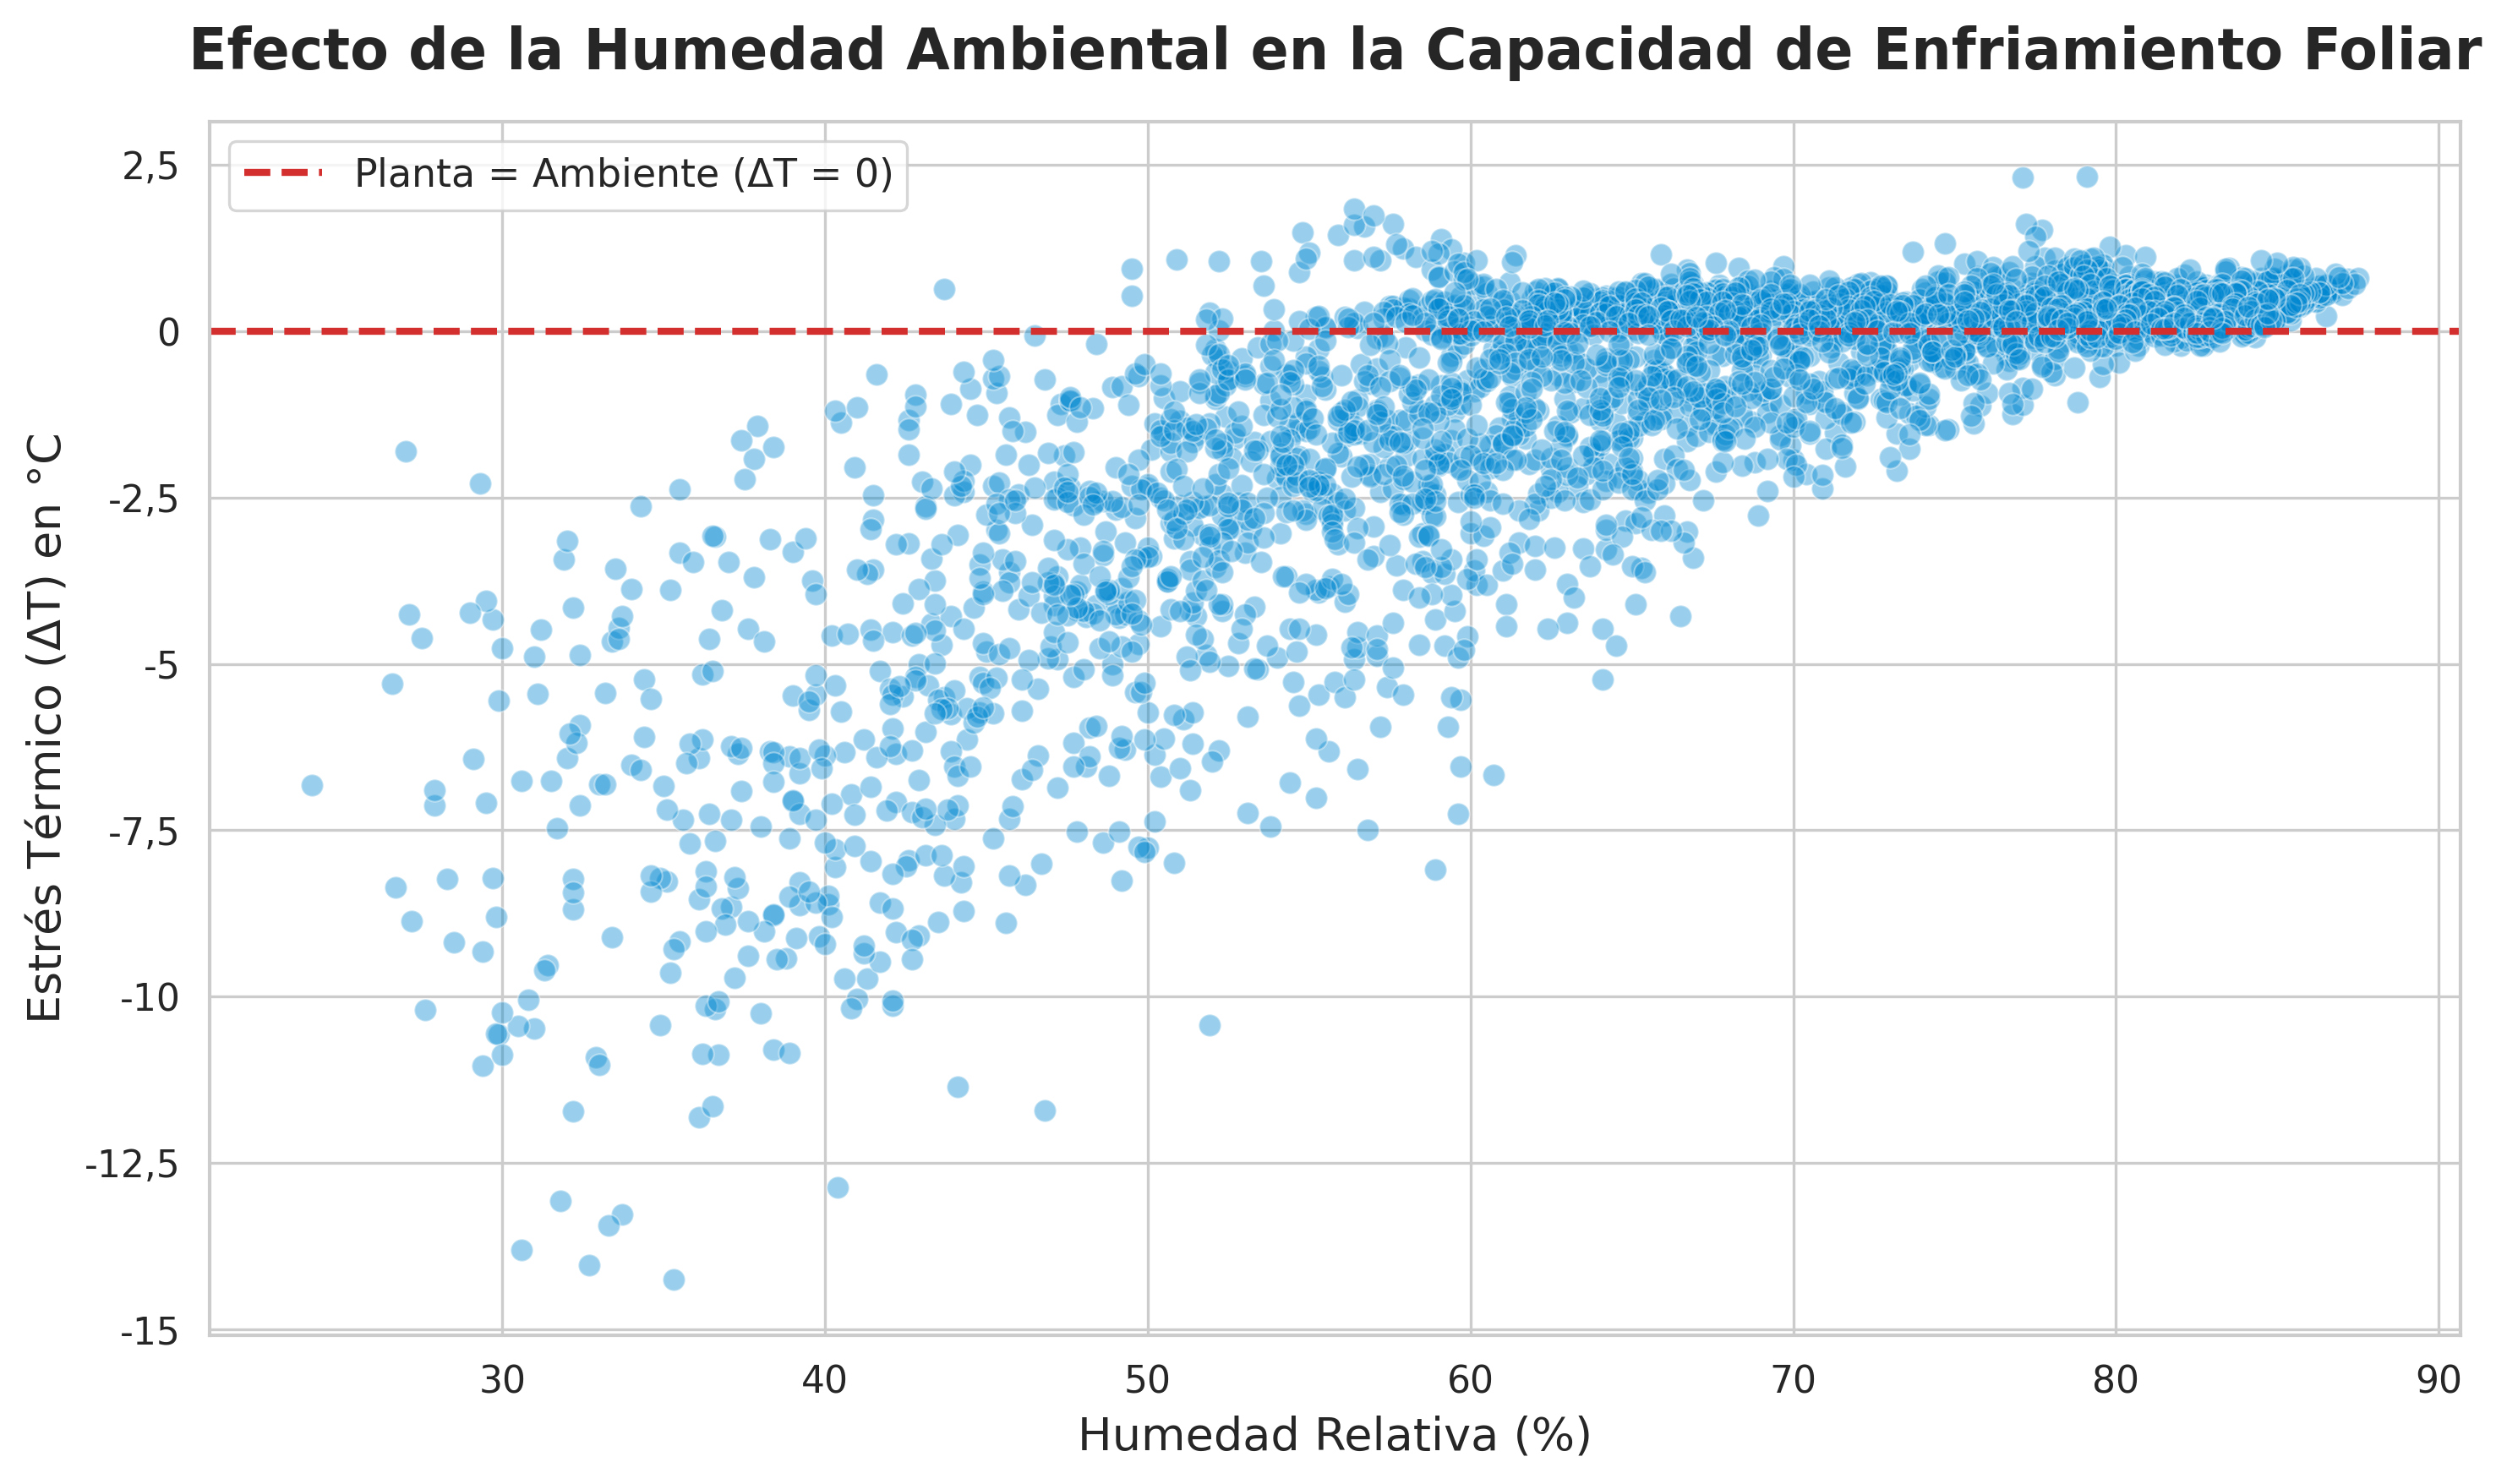
\includegraphics[width=0.8\textwidth]{img/humedad_vs_deltaT_academico.png}
    \label{fig:humedad_vs_deltaT}
    
    \vspace{0.2cm}
    \begin{minipage}{0.8\textwidth}
    \small{\textit{Nota:} El gráfico ilustra la limitación física que impone la humedad ambiental sobre la capacidad de refrigeración del dosel. A niveles de humedad superiores al $75\%$, los valores de $\Delta T$ convergen hacia $0$ °C, indicando que la transpiración se inhibe y la temperatura de la planta se acopla a la del aire circundante, independientemente de la carga por radiación solar o el riego.}
    \end{minipage}
\end{figure}
% --- FIN FIGURA 1 ---

% --- INICIO FIGURA 2 ---
\begin{figure}[H]
    \centering
    \caption{Dinámica del ciclo diurno de las variables micrometeorológicas y respuesta térmica foliar.}
    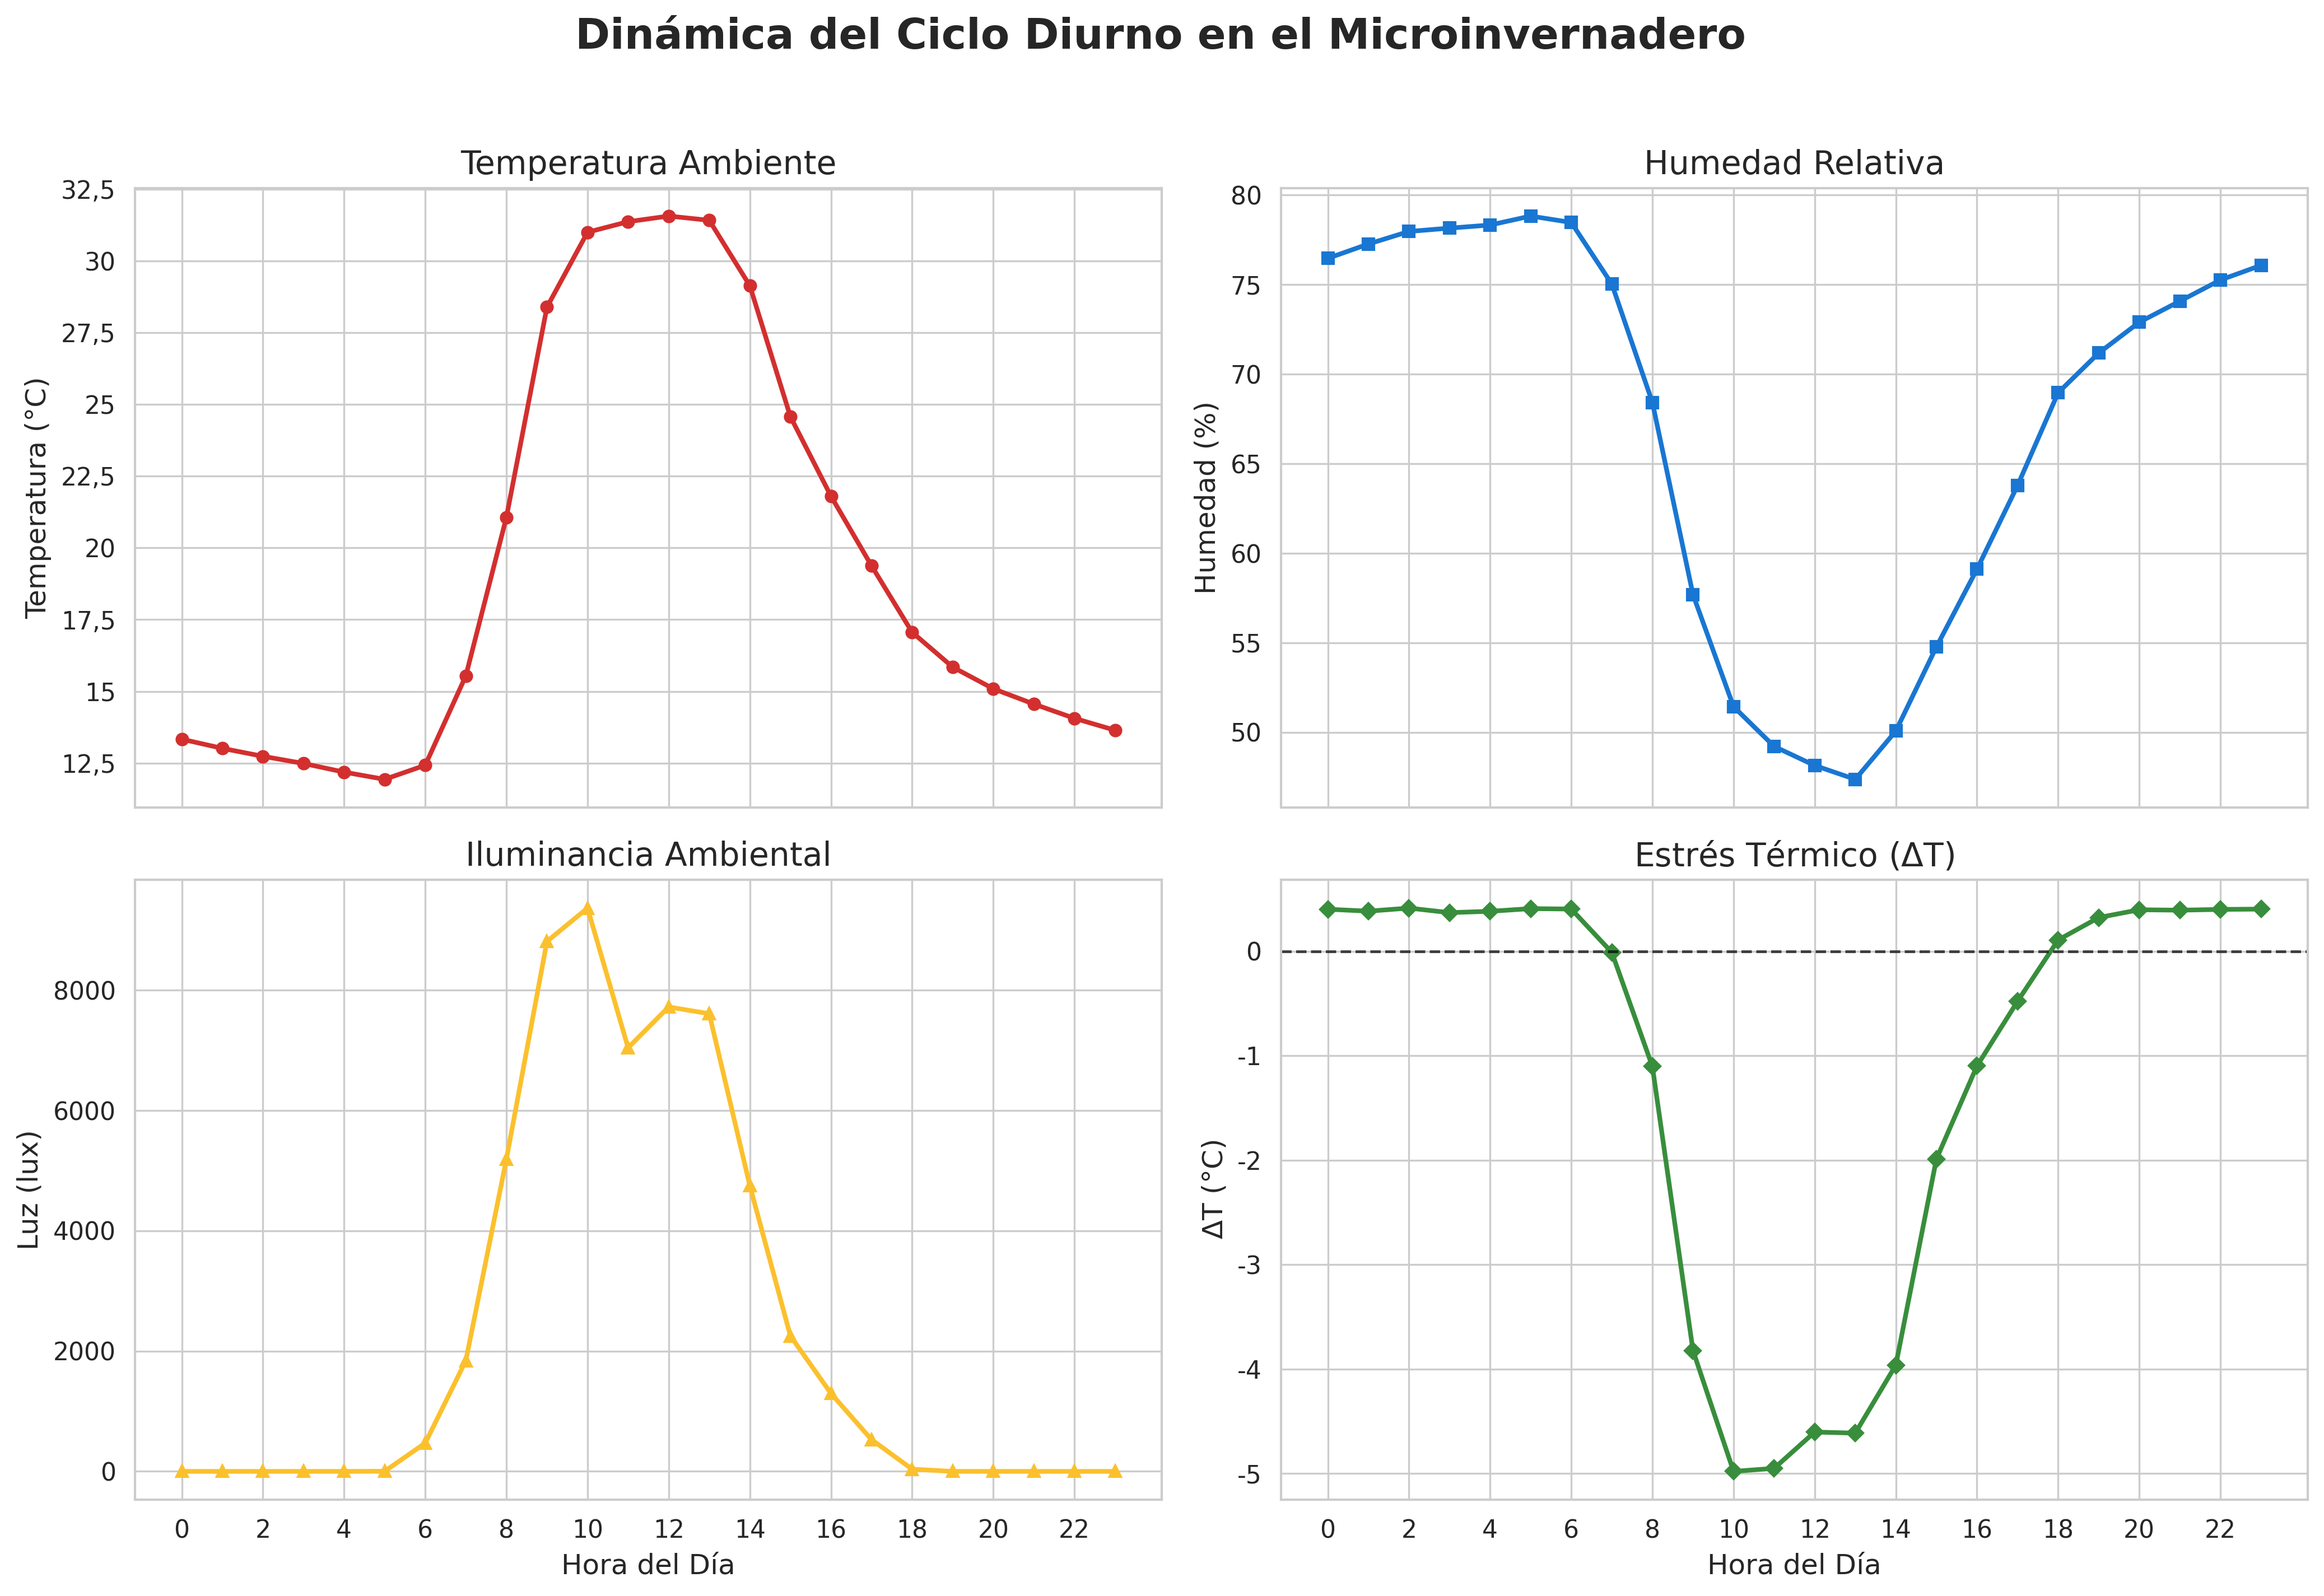
\includegraphics[width=\textwidth]{img/ciclo_diurno_academico.png}
    \label{fig:ciclo_diurno_invernadero}
    
    \vspace{0.2cm}
    \begin{minipage}{0.9\textwidth}
    \small{\textit{Nota:} El análisis agrupado por hora evidencia el comportamiento termodinámico del sistema. Se observa cómo el pico de iluminancia y temperatura (10:00 - 13:00) coincide con el máximo esfuerzo de enfriamiento de la planta ($\Delta T$ más negativo), marcando la franja horaria ideal para evaluar el estado hídrico.}
    \end{minipage}
\end{figure}
% --- FIN FIGURA 2 ---

En síntesis, la caracterización determinó que el microinvernadero es un entorno dominado por la radiación solar, donde la temperatura de la planta experimenta una fuerte dependencia frente a la humedad relativa. Estas conclusiones fueron fundamentales para el desarrollo del proyecto, ya que demostraron empíricamente que la termografía de bajo costo ($MLX90640$) es capaz de capturar la dinámica transpiratoria, siempre y cuando sus datos sean procesados de la mano con variables ambientales complementarias y dentro de ventanas de tiempo específicas.

\subsection{Análisis de ruido inducido por la inestabilidad del montaje}
\label{subsec:exp_analisis_ruido}

Después de recopilar el dataset con sujeto intracontrol, se realizó un experimento comparativo a mayor escala, en un invernadero más grande, diseñado para monitorear tres plantas de arándano simultáneamente: un individuo estresado, uno con riego óptimo y uno de control (Figura \ref{fig:montaje_comparativo}). Para lograrlo, se implementó un montaje físico suspendiendo las cámaras térmicas mediante un sistema de cuerdas frente a los especímenes. Sin embargo, el análisis exploratorio de este dataset (\textit{comparativo}) reveló inconsistencias críticas que obligaron a reconsiderar el diseño experimental hacia el modelo de caso único (intracontrol).

El fallo principal del experimento comparativo radicó en la inestabilidad micromecánica del montaje. La suspensión por cuerdas fue inestable, se desjustaba con frecuencia y esto generó un movimiento pendular continuo de las cámaras. Esto provocó el fracaso iterativo del algoritmo de segmentación térmica, introduciendo radiación de fondo (plastico de la pared, suelo y macetas) en el cálculo de la temperatura foliar.

La consecuencia de estos factores se evidencia en el análisis de dispersión y correlación (Figura \ref{fig:contraste_datasets}). En el dataset comparativo (fila superior), la contaminación por el fondo generó lecturas térmicas físicamente imposibles para el dosel (con máximos registrados de hasta 101,66 °C y valores de $\Delta T$ de 94,21 °C), destruyendo por completo la relación lineal esperada entre el índice CWSI y el gradiente térmico $\Delta T$. La correlación en este montaje inestable cayó a un deficiente $r = 0,12$.

\begin{figure}[H]
    \centering
    \caption{Montaje físico suspendido mediante cuerdas para el experimento comparativo.}
    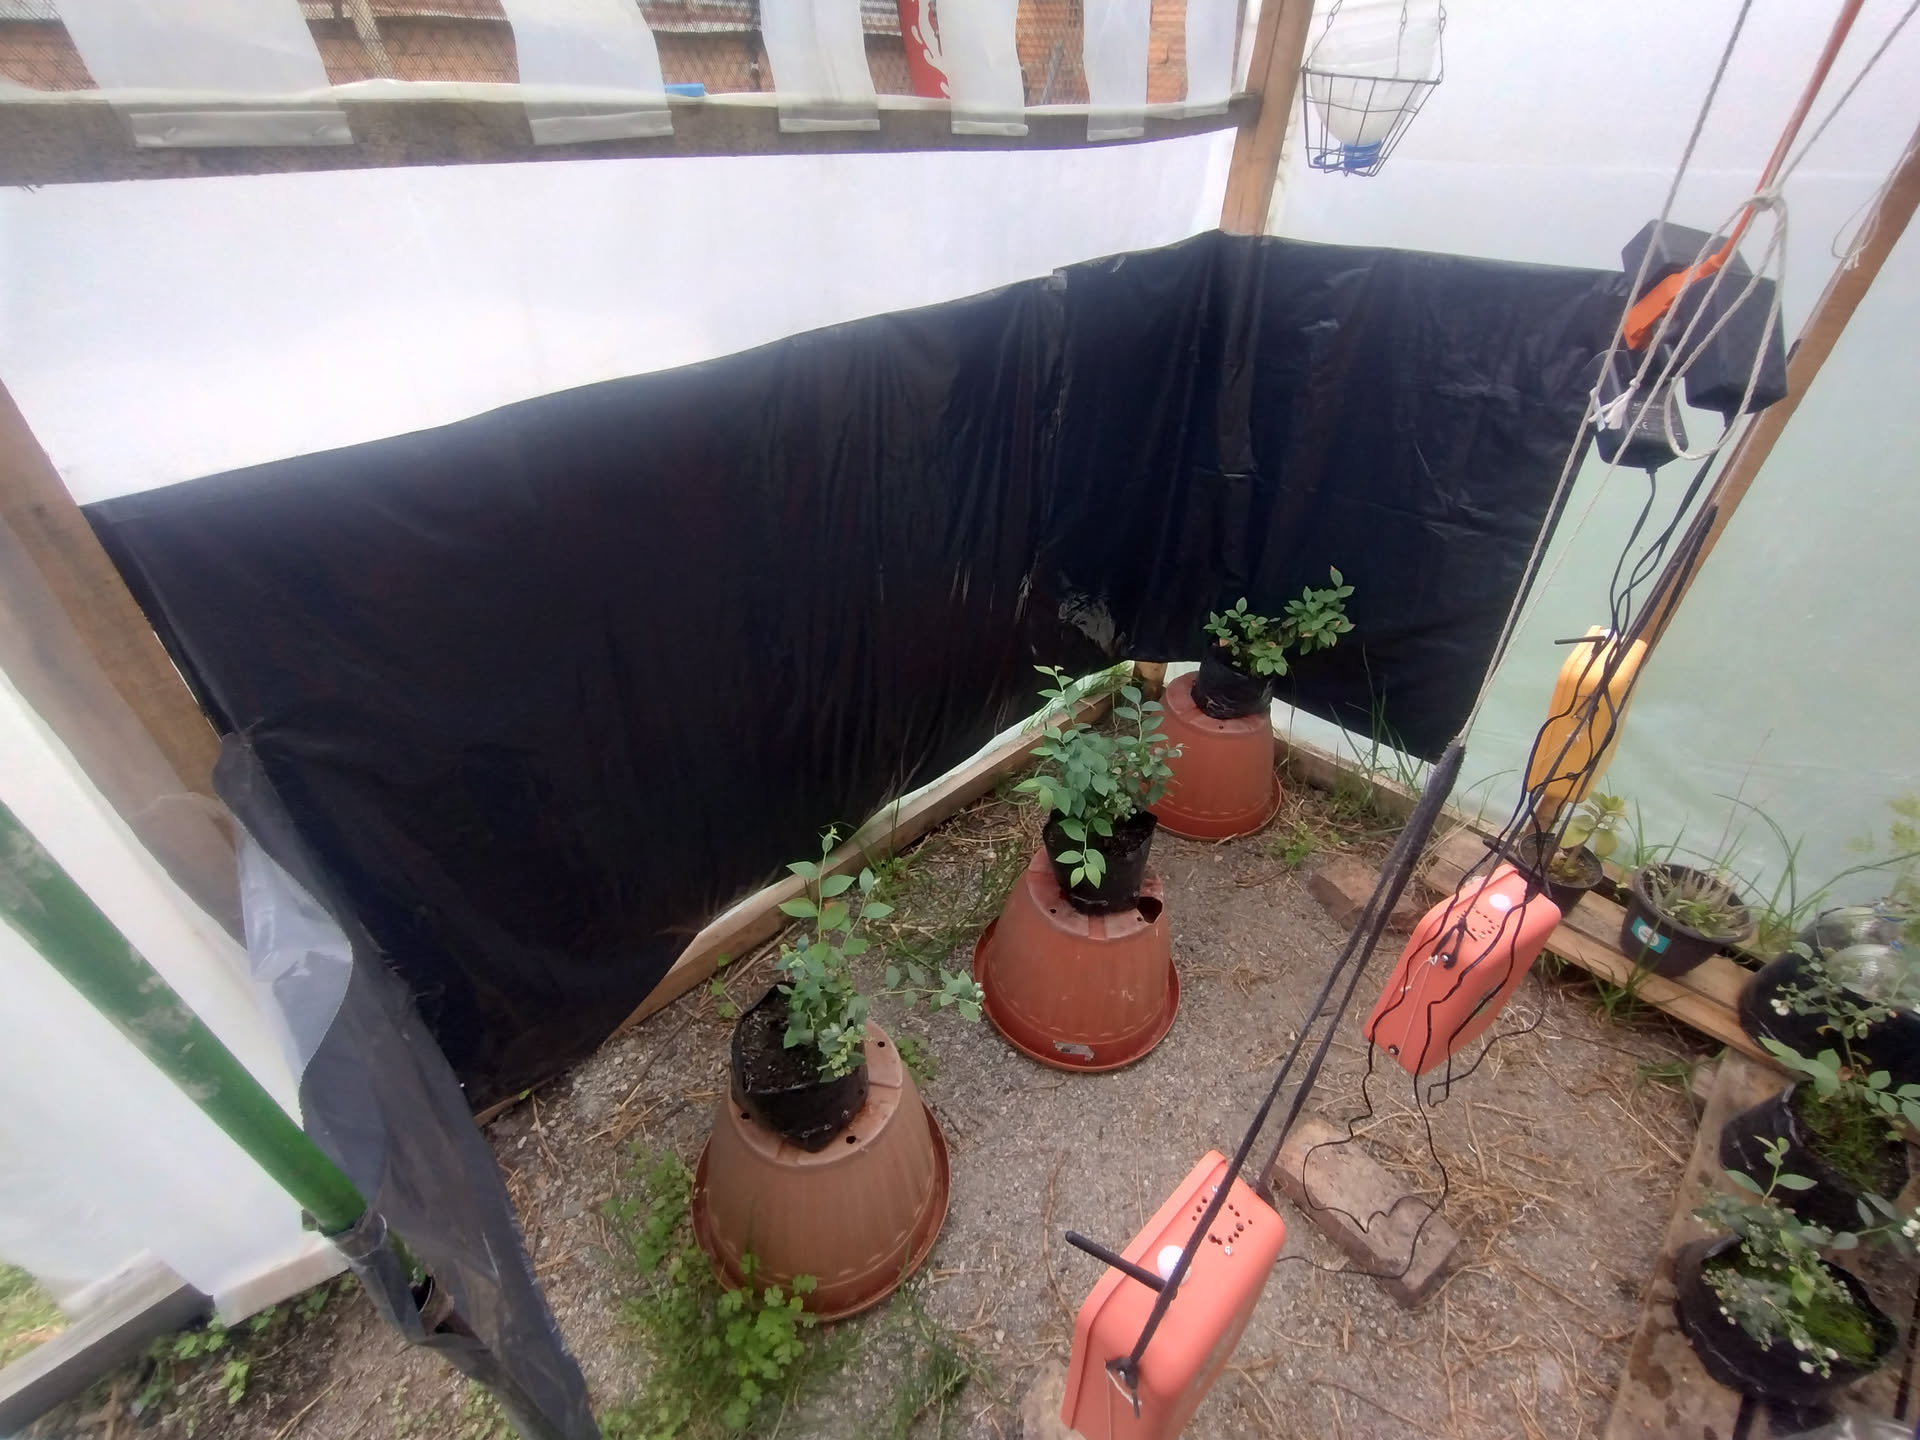
\includegraphics[width=0.95\textwidth]{img/montaje_comparativo.jpeg} 
    \label{fig:montaje_comparativo}
    
    \vspace{0.2cm}
    \begin{minipage}{0.8\textwidth}
    \small{\textit{Nota:} La imagen ilustra la disposición de las cámaras térmicas frente a los tres sujetos de estudio. Este sistema de sujeción introdujo inestabilidad mecánica que afectó la precisión de la segmentación foliar.}
    \end{minipage}
\end{figure}

% --- INICIO FIGURA CONTRASTE ---
\begin{figure}[H]
    \centering
    \caption{Contraste de dispersión y correlación: Dataset Comparativo vs. Dataset Empírico.}
    
    % Imagen del dataset malo (superior)
    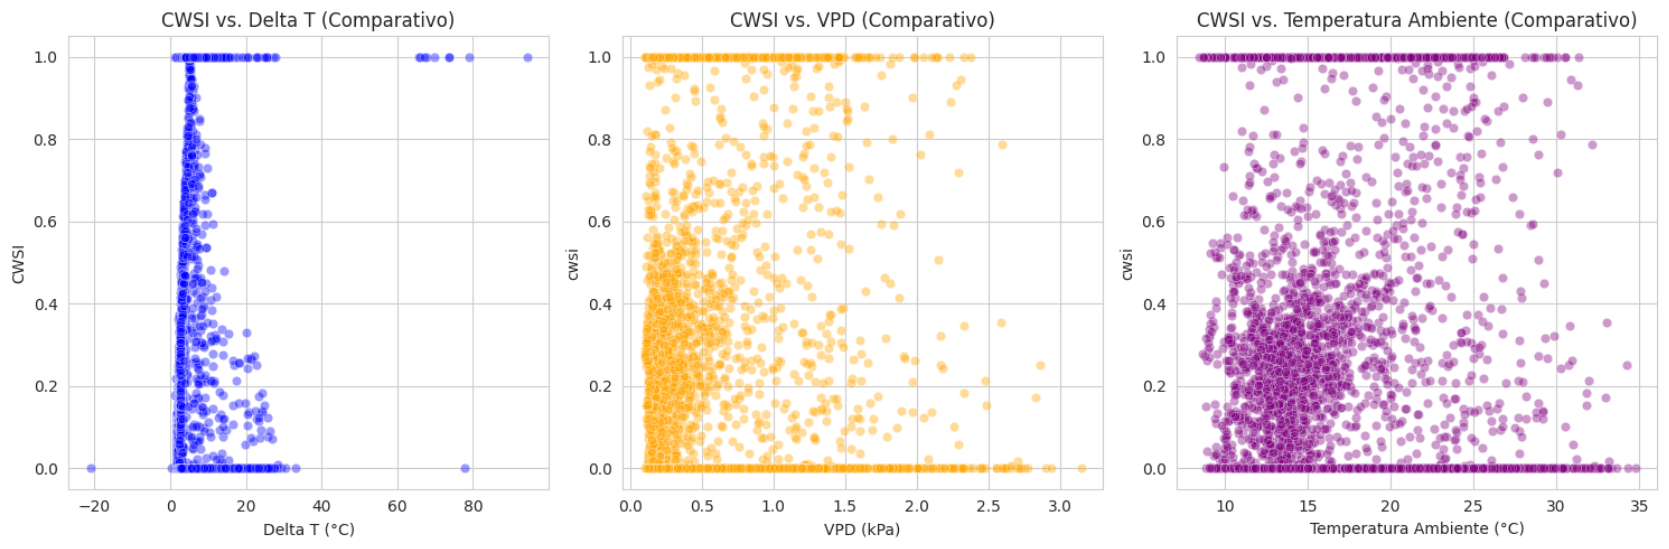
\includegraphics[width=\textwidth]{img/cwsi_comparativo.png} % Reemplaza con el nombre de tu primera imagen
    
    \vspace{0.5cm} % Espacio entre imágenes
    
    % Imagen del dataset bueno (inferior)
    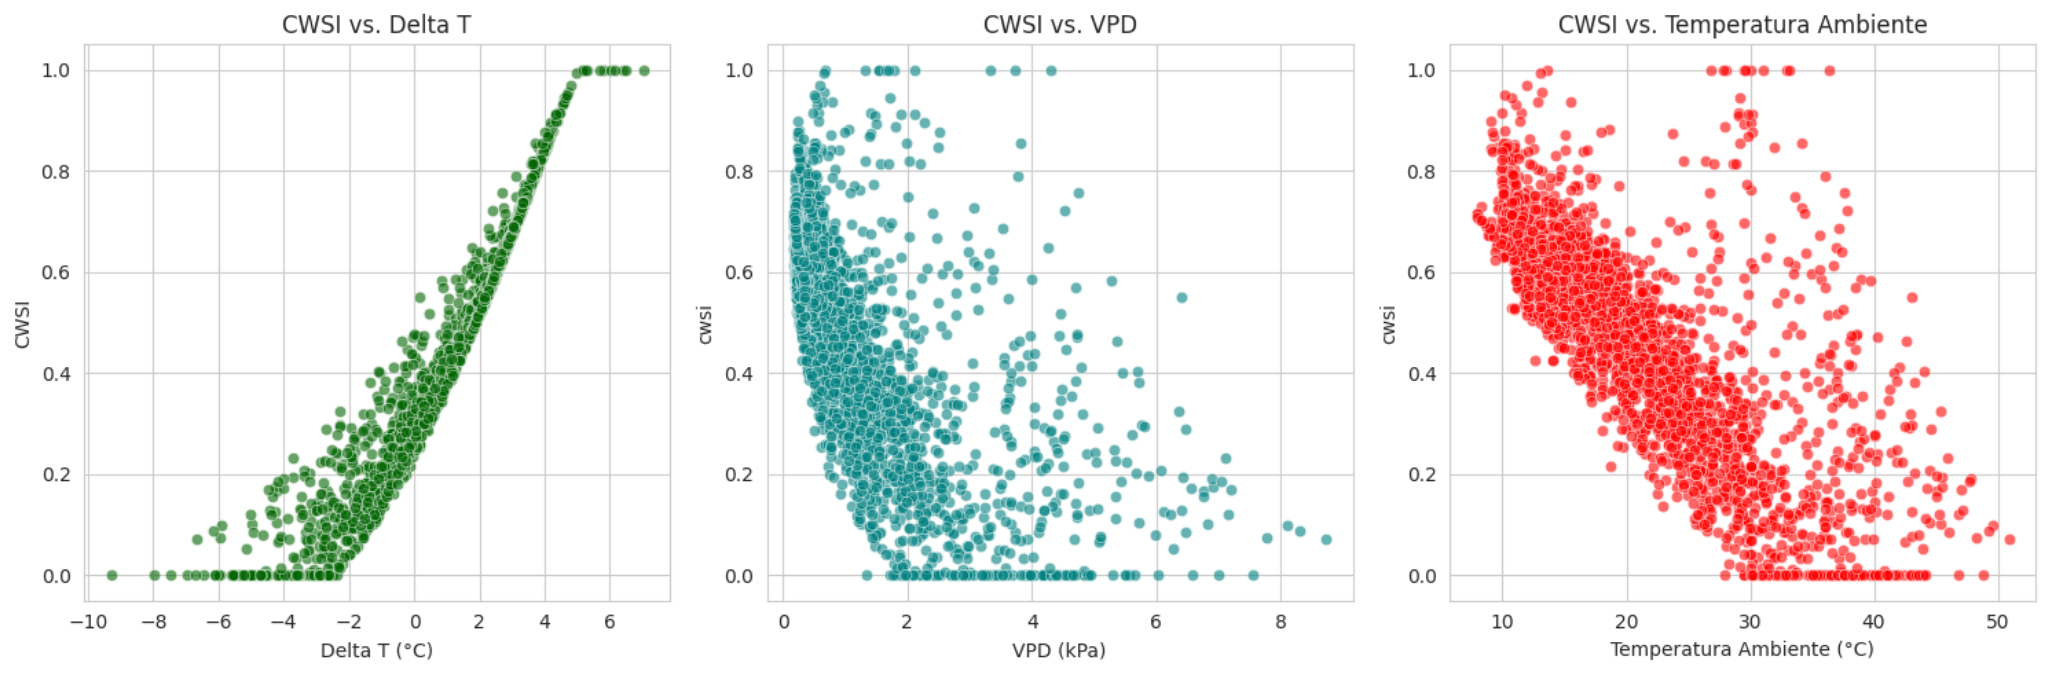
\includegraphics[width=\textwidth]{img/cwsi_empirico.png} % Reemplaza con el nombre de tu segunda imagen
    
    \vspace{0.2cm}
    \begin{minipage}{\textwidth}
    \small{\textit{Nota:} La fila superior muestra la dispersión anómala y la ausencia de correlación del experimento multi-planta debido a la contaminación del fondo y fallos de calibración. La fila inferior ilustra el comportamiento del experimento final (intracontrol estático), donde la estabilidad del montaje permitió capturar una relación termodinámica casi perfecta ($r = 0,96$) entre el CWSI y el diferencial térmico $\Delta T$.}
    \end{minipage}
    \label{fig:contraste_datasets}
\end{figure}
% --- FIN FIGURA CONTRASTE ---

En contraste, el diseño inicial de caso único ($n=1$), donde el sensor y la planta se mantuvieron rígidamente estáticos durante 55 días (fila inferior de la Figura \ref{fig:contraste_datasets}), permitió que el algoritmo de segmentación aislara satisfactoriamente el dosel. Los registros de temperatura máxima del follaje se mantuvieron dentro de límites biológicos coherentes (37,81 °C), restableciendo una correlación casi perfecta ($r = 0,96$) entre el $\Delta T$ y el CWSI calculado.

Estas lecciones aprendidas demuestran que, en sistemas de bajo costo con matrices de baja resolución como el MLX90640, la precisión micromecánica del montaje y la eliminación del ruido de fondo son factores tan críticos como la validación electrónica del propio sensor.

\section{Resultados}
\label{sec:exp_resultados}

Los resultados obtenidos con el sistema de monitoreo durante los 55 días permiten evaluar su capacidad para registrar la respuesta fisiológica de la planta de arándano (variedad Biloxi) ante el estrés hídrico inducido y su posterior recuperación.

La Figura \ref{fig:dist_horaria_deltaT} muestra la distribución de los valores de $\Delta T$ (Estrés Térmico: $T_{\text{canopia}} - T_{\text{aire}}$) capturados por el sistema a lo largo de las 24 horas del día, agrupando todos los datos del experimento. Se revela un patrón circadiano bien definido. Durante las horas nocturnas (aproximadamente 20:00 a 06:00), las mediciones de $\Delta T$ se mantienen estables y muy cercanas a $0^{\circ}$C, con una variabilidad mínima. Este comportamiento es coherente con el hecho de que, sin la energía de la radiación solar, la actividad de transpiración es casi nula y la planta alcanza un equilibrio térmico con su entorno \shortcite{GarciaTejero2015}.

% --- INICIO FIGURA 1 ---
\begin{figure}[H] % Usar [H] del paquete float si se ancló la tabla
    \centering
    \caption{Distribución horaria del estrés térmico ($\Delta T$).}
    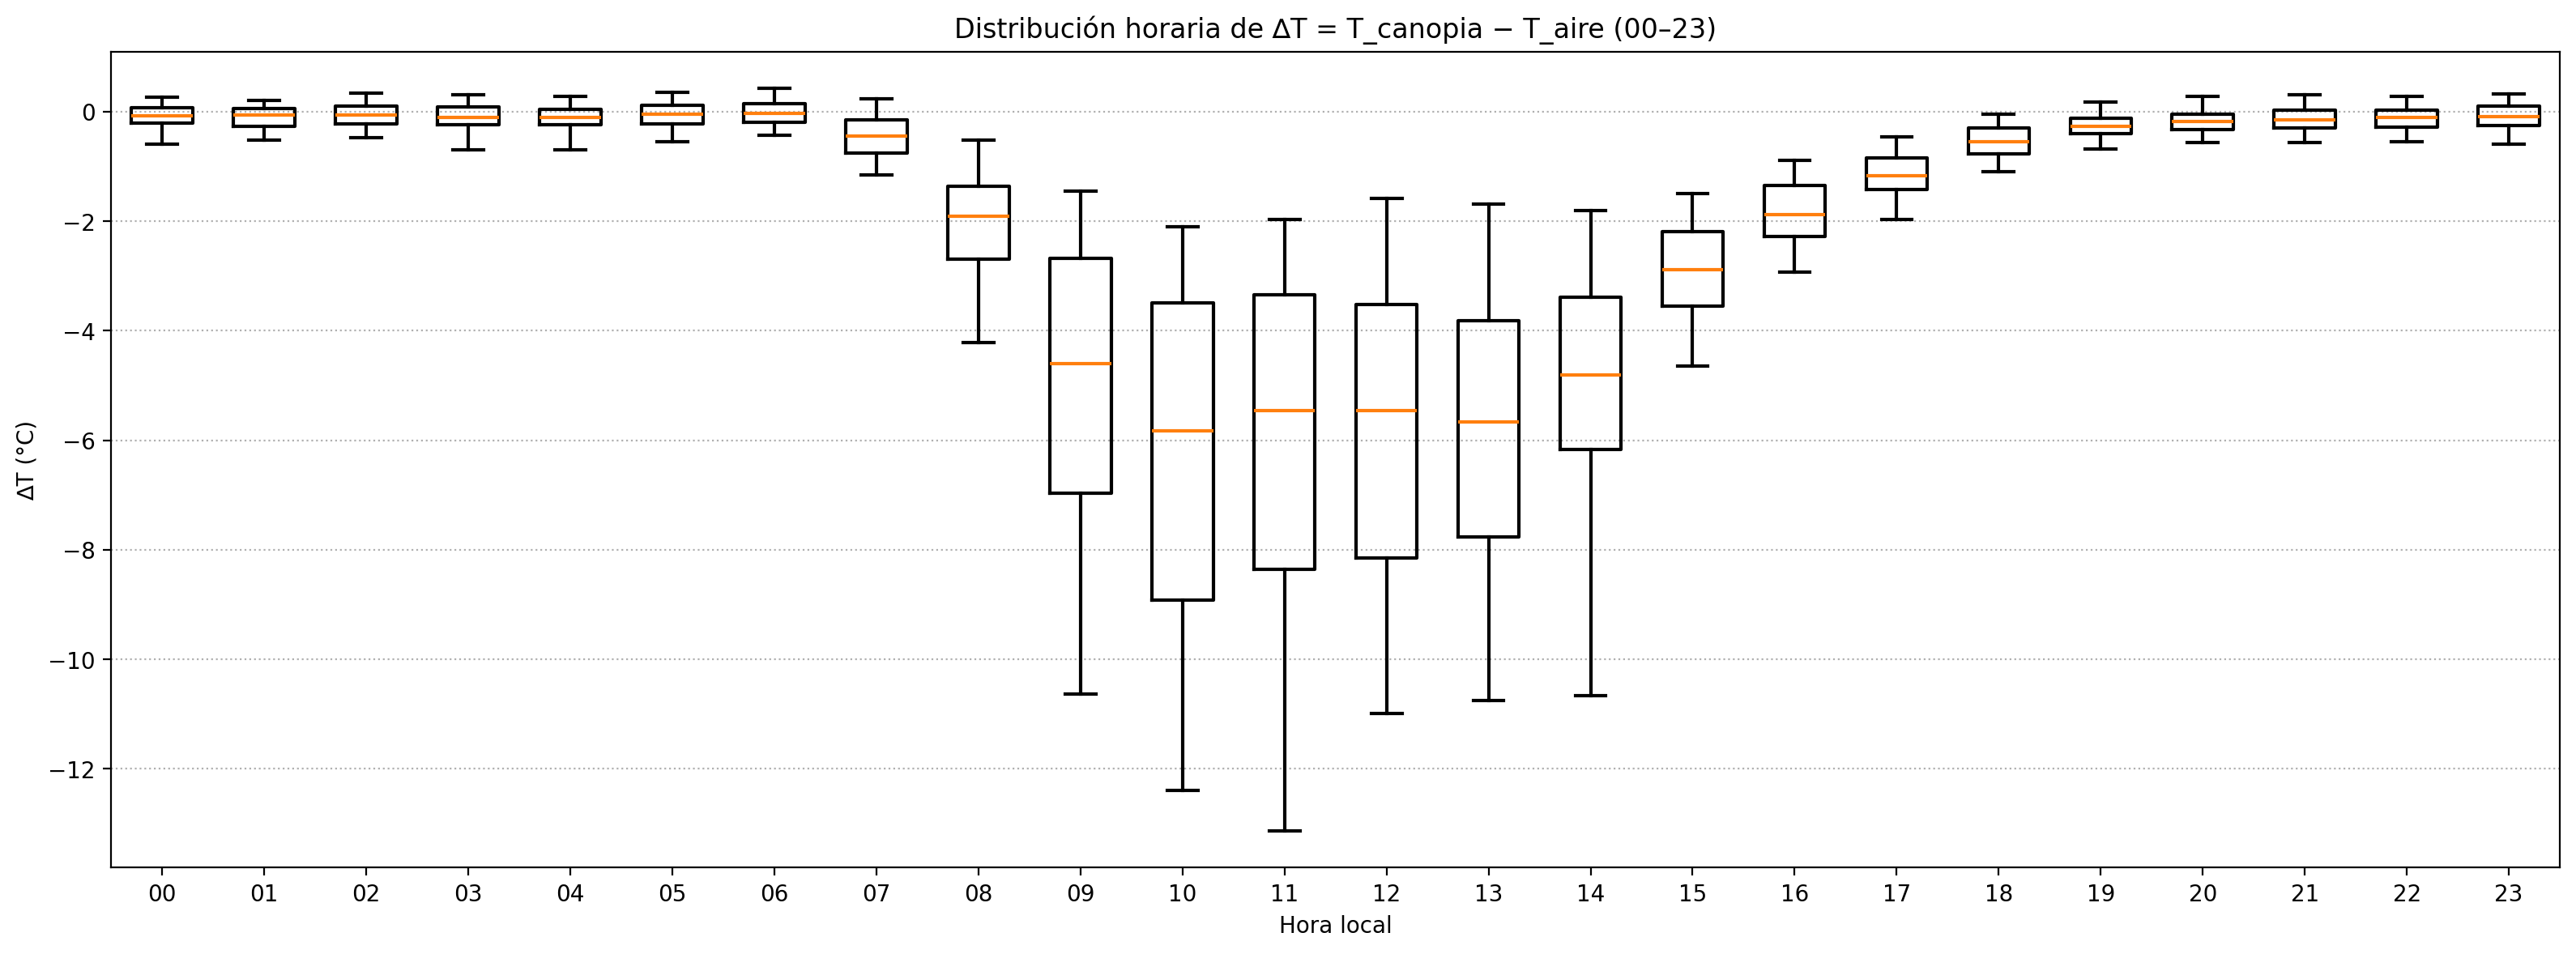
\includegraphics[width=1\textwidth]{img/deltaT_por_hora.png} 
    
    \vspace{0.2cm}
    \begin{minipage}{0.8\textwidth}
    \end{minipage} 
    \label{fig:dist_horaria_deltaT}
\end{figure}
% --- FIN FIGURA 1 ---

En las horas fotosintéticamente activas, a partir de las 07:00, el sistema registra un marcado descenso en los valores de $\Delta T$, indicando el inicio de la transpiración y el consecuente enfriamiento foliar. Este proceso se intensifica a lo largo de la mañana, y las medianas de $\Delta T$ alcanzan sus valores más negativos (por debajo de $-5^{\circ}$C) entre las 10:00 y las 13:00. Este comportamiento es consistente con el enfriamiento por evaporación, mecanismo vital mediante el cual la planta disipa la carga térmica impuesta por la radiación solar \shortcite{GarciaTejero2015}.

La característica más reveladora del gráfico es la gran variabilidad registrada durante este pico de actividad diurna (10:00-14:00), visible en la amplia dispersión de los datos (cajas y bigotes largos) y los valores extremos. Esta dispersión es crucial, ya que el gráfico agrupa los 55 días de datos, incluyendo tanto el periodo de estrés como el de recuperación. El valor mínimo registrado (aproximadamente $-13^{\circ}$C) representa la máxima capacidad de enfriamiento de la planta en días soleados y con riego óptimo. En contraste, el extremo superior de las cajas y bigotes (más cercano a $0^{\circ}$C) corresponde a los momentos en que la planta, bajo estrés hídrico severo, no podía transpirar eficazmente y su temperatura foliar se acercaba a la del aire. La captura de este amplio rango dinámico es la evidencia visual de que el sistema de bajo costo fue lo suficientemente sensible para registrar todo el espectro de respuestas fisiológicas de la planta, desde el riego óptimo hasta el estrés severo.

Si bien la captura de este rango valida la sensibilidad del sensor, un análisis más profundo requiere normalizar las mediciones para eliminar la influencia de las condiciones ambientales. Por ello, se utilizó el CWSI como métrica clave. La Figura \ref{fig:heatmap_cwsi} presenta un mapa de calor que visualiza la evolución diaria y horaria de este índice durante el experimento. Los colores cálidos (amarillo) indican un alto estrés (CWSI $\approx 1$) detectado por el sistema, y los colores fríos (morado/azul), un bajo estrés (CWSI $\approx 0$). La línea punteada horizontal señala el momento de la reanudación del riego (Día 46). Los puntos blancos indican datos faltantes por fallas técnicas menores.

% --- INICIO FIGURA 2 ---
\begin{figure}[H]
    \centering
    \caption{Mapa horario del índice de estrés hídrico del cultivo (CWSI) durante los 55 días del experimento.}
    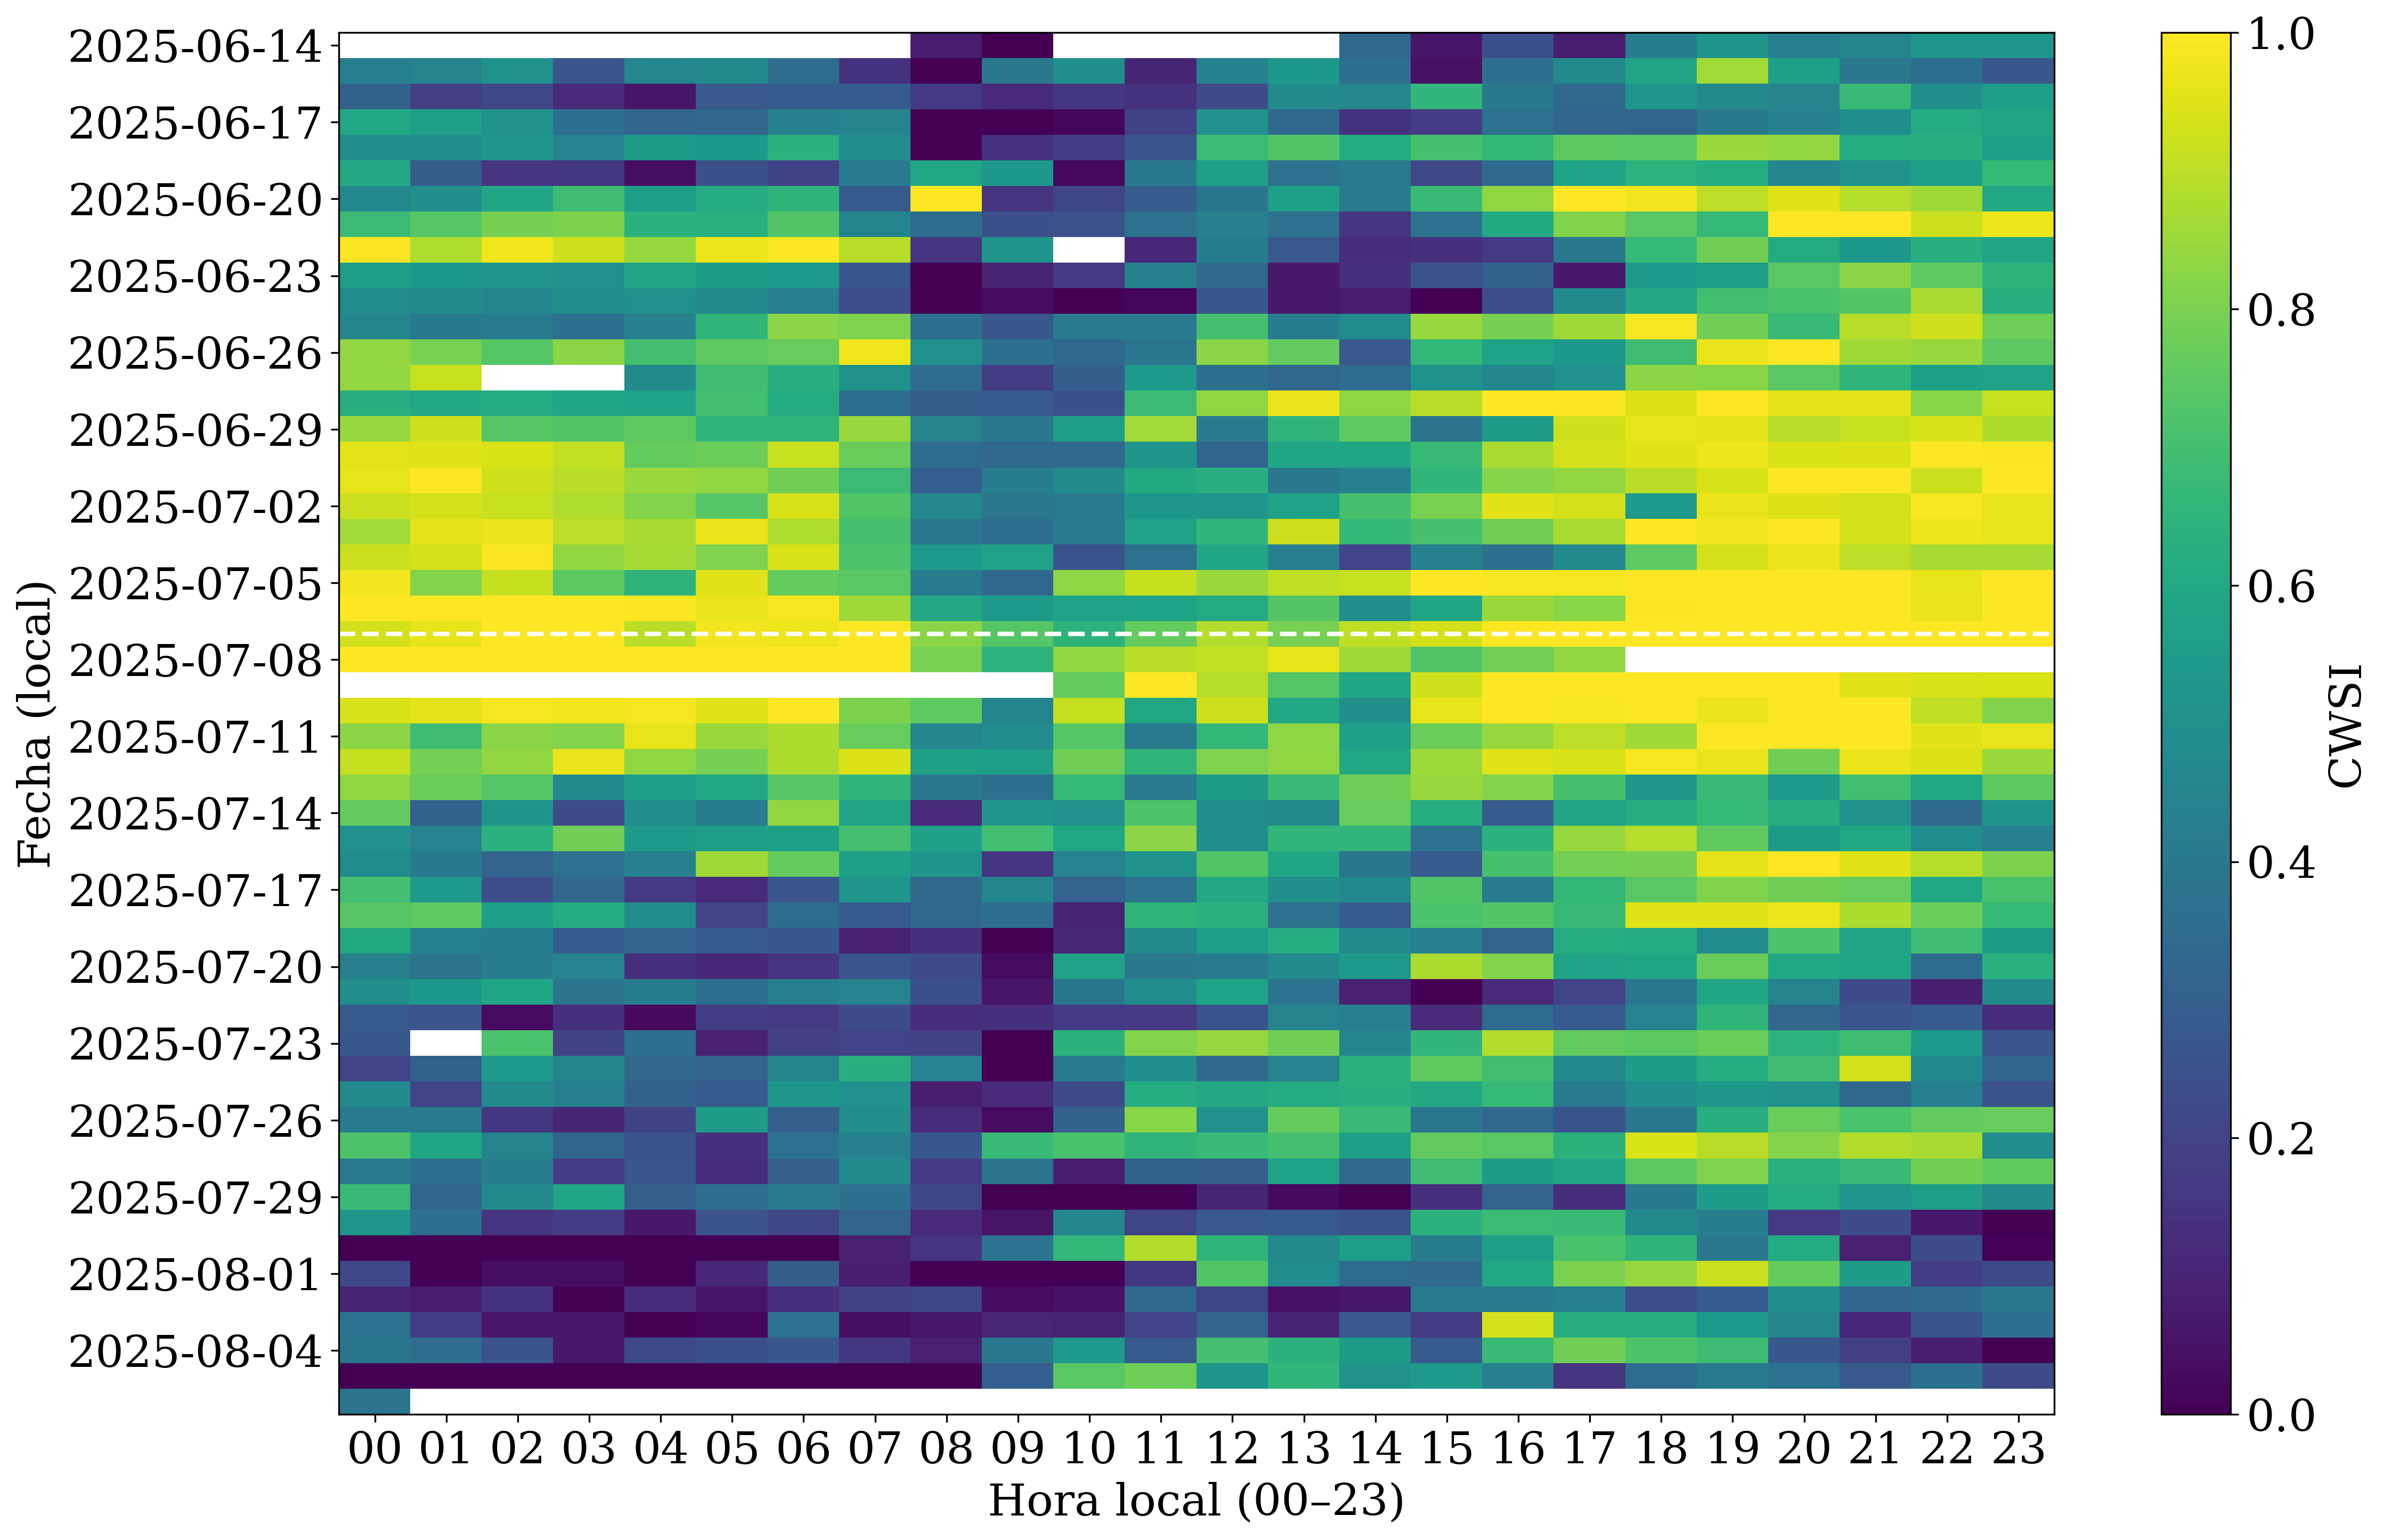
\includegraphics[width=\textwidth]{img/cwsi_horario.png}
    
    \vspace{0.2cm}
    \begin{minipage}{\textwidth}
    \end{minipage}
    \label{fig:heatmap_cwsi}
\end{figure}
% --- FIN FIGURA 2 ---

El mapa de calor demuestra claramente el funcionamiento del sistema. Durante el periodo de sequía inducida (antes de la línea punteada), el sistema registró consistentemente los valores más altos de CWSI (predominio de colores verdes/amarillos) durante las horas de máxima demanda atmosférica (aproximadamente 10:00-17:00). Tras la reanudación del riego (después de la línea punteada), se observa una transición vertical abrupta hacia colores fríos (morados/azules) en esas mismas horas, indicando una rápida recuperación del estado hídrico de la planta. Esta clara diferencia antes y después del riego valida la sensibilidad del sistema para detectar cambios en el estado hídrico a lo largo del tiempo. El aumento del CWSI durante la sequía es consecuencia directa de la reducción de la transpiración por cierre estomático \shortcite{Pineda2021}, mientras que el descenso post-riego refleja la reapertura estomática y la reanudación del enfriamiento \shortcite{Yu2015}.
Adicionalmente, el sistema capturó interacciones complejas. Se observan algunas noches con CWSI elevado durante la fase de sequía, sugiriendo estrés acumulado. Inversamente, algunas tardes muestran CWSI bajo, probablemente por eventos climáticos (lluvia, nubosidad) que enfrían externamente la hoja, ``enmascarando'' temporalmente el estrés interno \shortcite{Carolayn2020}. Dado que estas observaciones demuestran una fuerte dependencia entre las mediciones térmicas y el clima, se vuelve fundamental analizar esta relación. La Figura \ref{fig:deltaT_vs_clima} compara la distribución de $\Delta T$ bajo diferentes condiciones climáticas reportadas por la API externa.

% --- INICIO FIGURA 3 ---
\begin{figure}[H]
    \centering
    \caption{Distribución del estrés térmico ($\Delta T$) segmentado por condición climática externa.}
    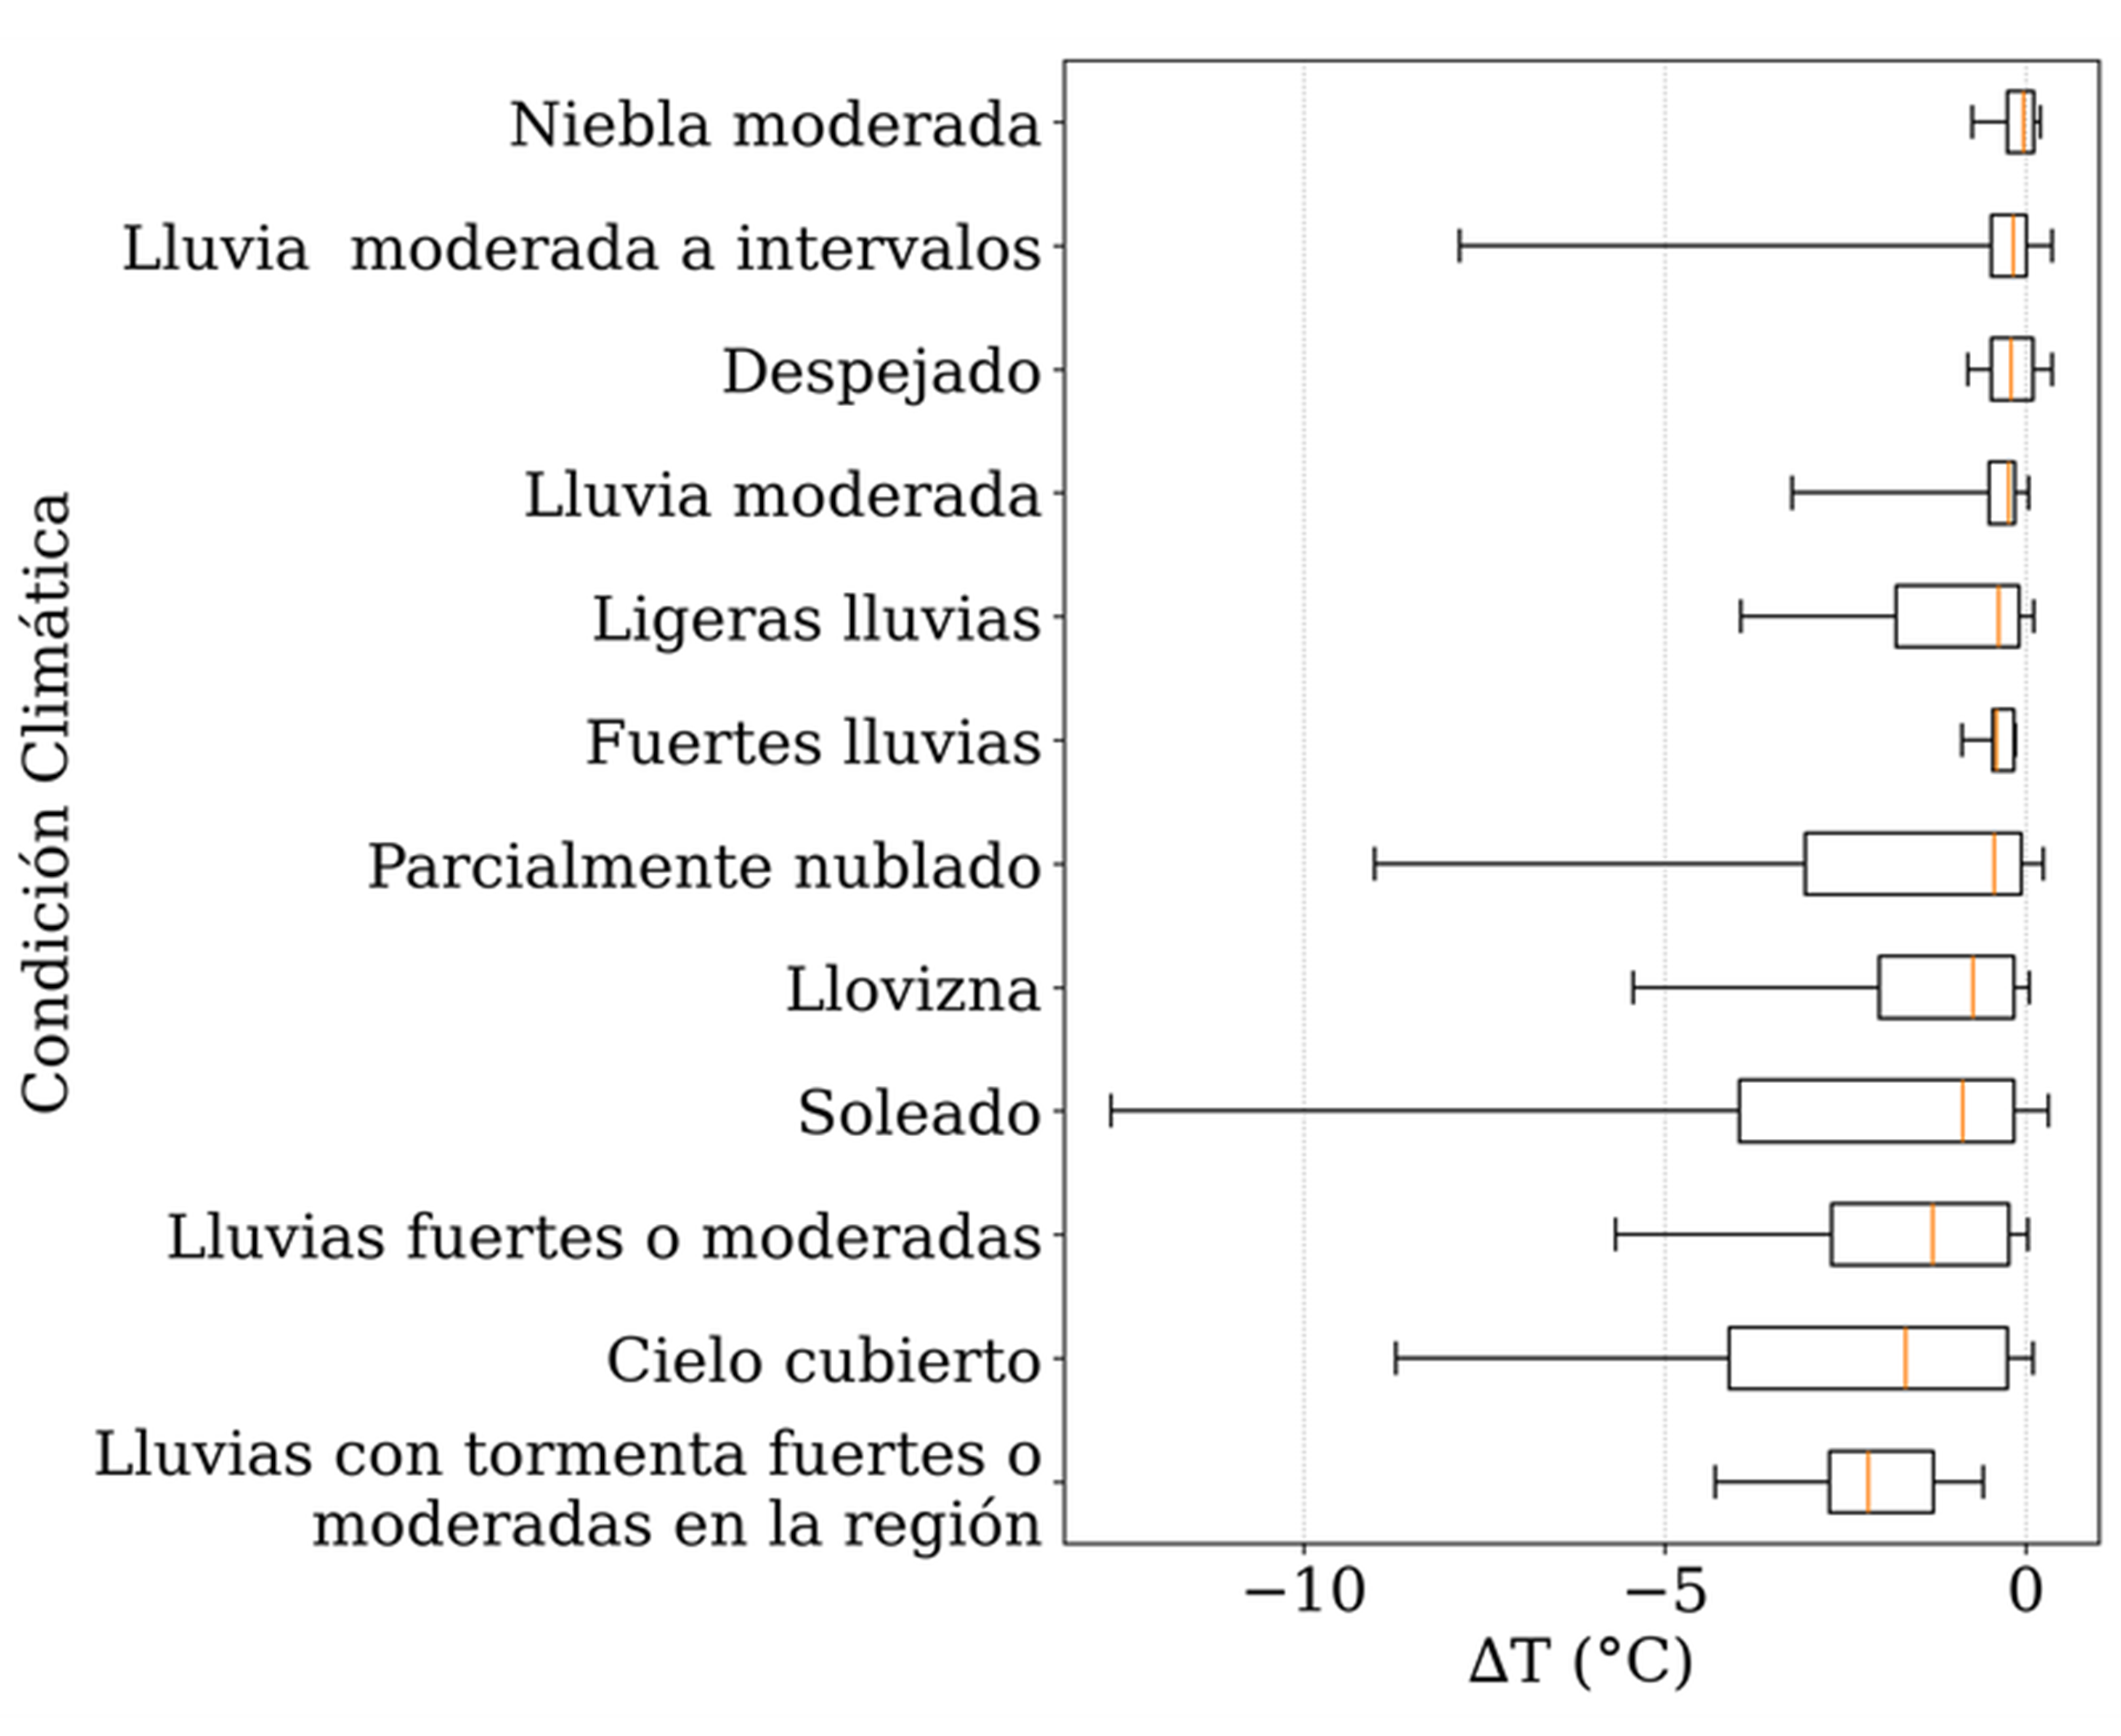
\includegraphics[width=0.8\textwidth]{img/clima.png}
    
    \vspace{0.2cm}
    \begin{minipage}{0.8\textwidth}
    \small{\textit{Nota:} Esta gráfica ilustra cómo influye el clima sobre el estrés térmico medido. En días despejados o soleados, el $\Delta T$ alcanza sus máximos y presenta mayor dispersión, mientras que en días nublados o lluviosos la diferencia de temperatura es menor y se mantiene estable, lo que reduce la variabilidad del índice.}
    \end{minipage}
    \label{fig:deltaT_vs_clima}
\end{figure}
% --- FIN FIGURA 3 ---


El gráfico muestra dos comportamientos opuestos. En condiciones de alta humedad y baja radiación ("Niebla moderada", "Lluvia"), los valores de $\Delta T$ se agrupan cerca de $0^{\circ}$C con mínima variabilidad, reflejando la limitación física de la transpiración en aire saturado. Por el contrario, en días de alta radiación ("Soleado", "Despejado"), el sistema registra la máxima capacidad de enfriamiento ($\Delta T$ medianos $<-5^{\circ}$C, mínimos $\approx -12^{\circ}$C) y la mayor variabilidad, que representa la diferencia entre la planta estresada y la bien regada bajo esas condiciones. Este gráfico (Figura \ref{fig:deltaT_vs_clima}) ilustra que las mediciones térmicas no pueden interpretarse aisladamente y valida la necesidad de usar índices normalizados como el CWSI o análisis segmentados por demanda atmosférica (VPD) \shortcite{Pineda2021}.

Tras establecer la fuerte dependencia de las mediciones térmicas con el clima en la Figura \ref{fig:deltaT_vs_clima}, la Tabla \ref{tab:deltaT_vs_VPD} ofrece un análisis cuantitativo más riguroso. Esta presenta una comparación del $\Delta T$ promedio medido por el sistema entre el periodo de ``Estrés Hídrico'' y el de ``Recuperación'', segmentado por rangos equivalentes de Déficit de Presión de Vapor (VPD).

% --- INICIO TABLA 1 ---
\FloatBarrier
\begin{table}[h!]
    \centering
    \caption{Comparación del estrés térmico ($\Delta T$) bajo demandas atmosféricas equivalentes.}
    \label{tab:deltaT_vs_VPD}
    \small % Hace la fuente un poco más pequeña si es necesario
    \begin{tabular}{c c c c c}
        \toprule
        \textbf{Rango VPD} & \multicolumn{2}{c}{\textbf{Estrés Hídrico}} & \multicolumn{2}{c}{\textbf{Recuperación}} \\
        \cmidrule(lr){2-3} \cmidrule(lr){4-5}
        \textbf{(kPa)} & \textbf{$\Delta T$ Promedio (°C)} & \textbf{N Muestras} & \textbf{$\Delta T$ Promedio (°C)} & \textbf{N Muestras} \\
        \midrule
        {[}0,0; 0,5) & 0,31 & 685 & 0,07 & 930 \\
        {[}0,5; 1,0) & -0,38 & 438 & -0,46 & 432 \\
        {[}1,0; 1,5) & -1,89 & 174 & -2,14 & 238 \\
        {[}1,5; 2,0) & -2,89 & 85 & -3,25 & 139 \\
        {[}2,0; 2,5) & -4,16 & 61 & -4,19 & 93 \\
        {[}2,5; 3,0) & -5,26 & 36 & -5,20 & 51 \\
        {[}3,0; 3,5) & -6,55 & 22 & -6,19 & 28 \\
        {[}3,5; 4,0) & -6,08 & 21 & -6,83 & 33 \\
        {[}4,0; 4,5) & -7,20 & 22 & -7,45 & 24 \\
        {[}4,5; 5,0) & -8,00 & 13 & -7,75 & 17 \\
        {[}5.0, 5.5) & -8,41 & 4 & -9,68 & 15 \\
        {[}5.5, 6.0) & -8,26 & 2 & -9,11 & 12 \\
        {[}6.0, 6.5) & -9,89 & 4 & -10,15 & 7 \\
        {[}6.5, 7.0) & -9,34 & 5 & -11,15 & 3 \\
        {[}7.0, 7.5) & -10,44 & 1 & -10,66 & 3 \\
        {[}7.5, 8.0) & N/A & N/A & -13,47 & 2 \\
        {[}8.0, 8.5) & N/A & N/A & -13,36 & 2 \\
        {[}8.5, 9.0) & N/A & N/A & -13,71 & 1 \\
        \bottomrule
    \end{tabular}
    \vspace{0.5em}
    \begin{minipage}{0.9\textwidth}
    \small{\textit{Nota:} Al seleccionar horas con condiciones de temperatura y humedad ambiental similares, se aísla el impacto directo de la disponibilidad hídrica. La tabla evidencia que, ante la misma presión climática (Demanda Evaporativa), la planta hidratada (fase de recuperación) mantiene su dosel considerablemente más fresco que durante el periodo de sequía severa.}
    \end{minipage}
\end{table}
\FloatBarrier
% --- FIN TABLA 1 ---

\bigskip

El análisis revela tres zonas de comportamiento que, en conjunto, validan la capacidad del sistema para detectar el estado hídrico:
\begin{itemize}
    \item \textbf{Zona de evidencia consistente (VPD < 2,5 kPa):} En condiciones de baja a moderada demanda atmosférica, donde se concentra la mayoría de las observaciones, los datos indican que el $\Delta T$ promedio registrado en la planta estresada es sistemáticamente más alto (menos negativo) que en la planta en recuperación. Esta diferencia, que es consistente con una menor capacidad de enfriamiento, refleja el principio básico de la termografía: el cierre estomático bajo estrés reduce la transpiración y eleva la temperatura foliar \shortcite{GarciaTejero2015}.
    \item \textbf{Zona de transición y ruido estadístico (VPD 2.5-5,0 kPa):} En este rango, las diferencias de $\Delta T$ se reducen e incluso se invierten. Este comportamiento se atribuye a dos factores combinados: la escasa cantidad de muestras en esta franja (que aumenta la incertidumbre estadística) y los límites fisiológicos del arándano. Con una demanda atmosférica muy alta, incluso una planta bien regada puede tener dificultades para absorber agua a la misma velocidad que la transpira, debido a su sistema radicular superficial \shortcite{Morales2017, Salgado2018}. Esto provoca que la respuesta térmica de la planta en ambas fases (estresada y en recuperación) converja, reduciendo la claridad de la señal en estas condiciones extremas y poco frecuentes.
    \item \textbf{Zona de tendencia sugerida (VPD > 5,0 kPa):} En este rango extremo, los datos son escasos para establecer conclusiones definitivas, pero sugieren una tendencia interesante. Mientras la planta en recuperación alcanzó un enfriamiento máximo ($\Delta T$ de hasta -13,71 $^{\circ}$C), la ausencia de registros para la planta estresada en las condiciones más severas apunta a un posible cierre estomatal casi total como mecanismo de supervivencia para evitar la deshidratación \shortcite{Yu2015}. Esto sugiere que es precisamente bajo esta alta exigencia donde la diferencia entre un estado hídrico saludable y uno deficiente se vuelve más pronunciada, destacando el potencial del sistema para detectar estrés severo.
\end{itemize}
Estos resultados cuantitativos, segmentados por VPD, refuerzan la validación de la sensibilidad del sistema para detectar diferencias en el estado hídrico bajo condiciones ambientales comparables.

